\documentclass[border=5pt]{standalone}
\usepackage{tikz}
\usepackage{amsmath}
\usetikzlibrary{calc, positioning, arrows.meta, 3d}
\begin{document}
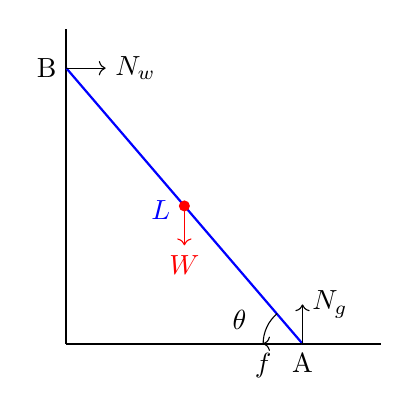
\begin{tikzpicture}[scale=1]
% Draw wall
\draw[thick] (0,0) -- (0,4);
% Draw ground
\draw[thick] (0,0) -- (4,0);
% Draw ladder
\draw[thick, blue] (0,3.5) -- (3,0);
% Mark angle
\draw (2.5,0) arc (180:130:0.5);
\node at (2.2,0.3) {$\theta$};
% Mark length
\node[blue] at (1.2,1.7) {$L$};
% Mark weight at center
\fill[red] (1.5,1.75) circle (2pt);
\draw[red, ->] (1.5,1.75) -- (1.5,1.25) node[below] {$W$};
% Mark forces
\draw[->] (0,3.5) -- (0.5,3.5) node[right] {$N_w$};
\draw[->] (3,0) -- (3,0.5) node[right] {$N_g$};
\draw[->] (3,0) -- (2.5,0) node[below] {$f$};
% Labels
\node[below] at (3,0) {A};
\node[left] at (0,3.5) {B};
\end{tikzpicture}
\end{document}
